\chapter{البوليمرات}\label{ch:g12:polymers}

يمكن غزل سترة صوفية صناعية من قوارير مشروبات مصهورة؛ وحبل التسلق
مصنوع من النايلون؛ وهذه الصفحة سليلوز، صنعته الأشجار. وكل هذه الثلاثة
\omterm{def:g12:polymers:polymer}{بوليمرات}: \omterm{def:g7:atoms-and-molecules:molecule}{جزيئات} طولها آلاف \omterm{def:g7:atoms-and-molecules:atom}{الذرات}، مبنية بتكرار وحدة صغيرة
واحدة مرة بعد مرة. وخواصها --- لينة أو صلبة، مرنة أو
هشة، قابلة للصهر أو لا --- تأتي من \omterm{def:g7:atoms-and-molecules:atom}{الذرات} التي تحويها أقل مما
تأتي من طريقة ترتيب سلاسلها الطويلة.

\begin{recall}
\omterm{def:g8:plastics:plastic}{البلاستيك} مصنوع من \omterm{def:g7:atoms-and-molecules:molecule}{جزيئات} طويلة جدًا؛ فاللدائن الحرارية تلين بالتسخين،
واللدائن المتصلدة بالحرارة لا تلين (\cref{ch:g8:plastics}). مجموعات \omterm{def:g11:functional-groups:alcohol}{الكحول} والحمض \omterm{def:g11:functional-groups:carboxylic-acid}{والإستر}
\omterm{def:g11:functional-groups:amine}{والأمين} \omterm{def:g11:functional-groups:amine}{والأميد} (\cref{ch:g11:functional-groups}). والإضافة
تضم جزيئين في \omterm{def:g7:atoms-and-molecules:molecule}{جزيء} واحد دون أن تفقد أي \omterm{def:g7:atoms-and-molecules:atom}{ذرة}
(\cref{ch:g12:curly-arrows}).
\end{recall}

\begin{omfigure}
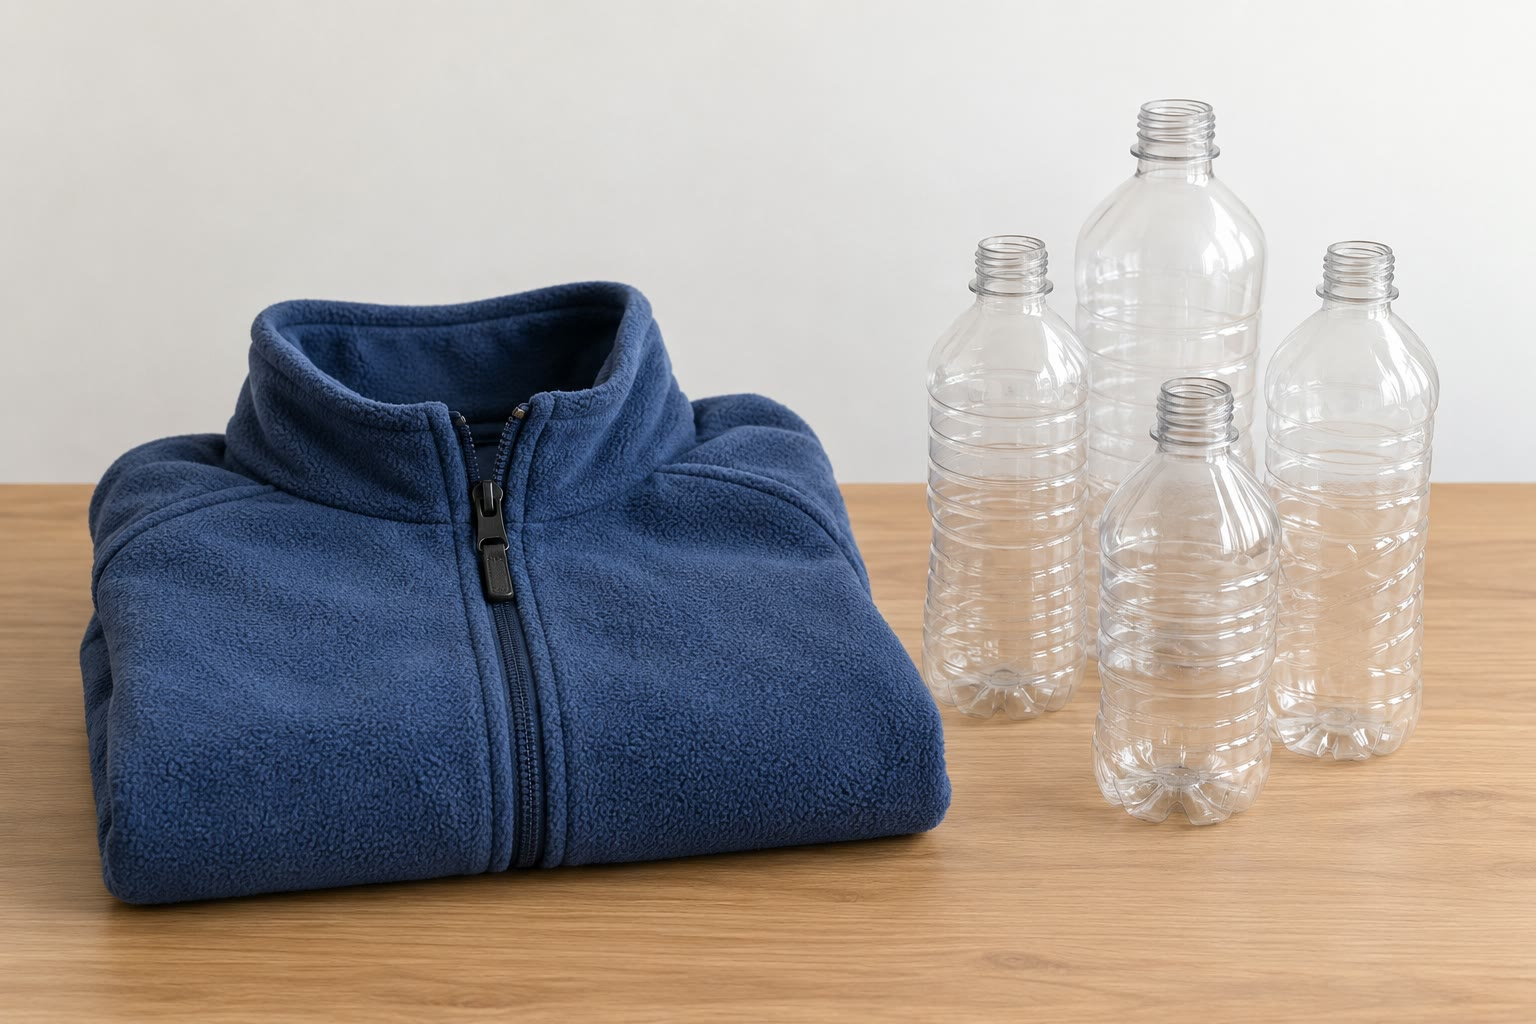
\includegraphics[width=0.45\linewidth]{images/book1/ai/g12-fleece-bottles.jpg}

{\small قوارير مشروبات مستعملة وسترة صوفية صناعية: \omterm{def:g12:polymers:polymer}{البوليمر} نفسه، في
شكلين.}
\end{omfigure}

\section{المونومرات والبوليمرات والوحدات المتكررة}

\begin{definition}[البوليمر، المونومر، البلمرة]\label{def:g12:polymers:polymer}
\emph{البوليمر}\index{بوليمر} مادة مكوّنة من \omterm{def:g7:atoms-and-molecules:molecule}{جزيئات} كبيرة
جدًا، هي \omterm{def:g7:atoms-and-molecules:molecule}{الجزيئات} الضخمة، كلٌّ منها مبني من وحدات صغيرة كثيرة مرتبطة
واحدةً بعد أخرى. \omterm{def:g7:atoms-and-molecules:molecule}{والجزيئات} الصغيرة التي يُصنع منها هي
\emph{مونومراته}\index{مونومر}؛ والتفاعل الذي يربطها هو
\emph{البلمرة}\index{بلمرة}.
\end{definition}

\begin{definition}[الوحدة المتكررة، درجة البلمرة]\label{def:g12:polymers:repeat-unit}
\emph{الوحدة المتكررة}\index{وحدة متكررة} في \omterm{def:g12:polymers:polymer}{البوليمر} هي أصغر
مجموعة من \omterm{def:g7:atoms-and-molecules:atom}{الذرات} يعطي تكرارها السلسلة؛ وتُكتب بين
قوسين معقوفين مع دليل $n$. والعدد $n$ للوحدات المتكررة في سلسلة هو
\emph{درجة بلمرتها}\index{درجة البلمرة}.
\end{definition}

\begin{omfigure}
\[
  n\;\ce{CH2=CH2}
  \quad\longrightarrow\quad
  \chemfig{-[@{op1,.75}]CH_2-CH_2-[@{cl1,0.25}]}
  \polymerdelim[height=6pt, depth=6pt, indice=n]{op1}{cl1}
\]

{\small \omterm{def:g12:polymers:polymer}{بلمرة} الإيثين: $n$ جزيئًا من \omterm{def:g12:polymers:polymer}{المونومر} تعطي سلسلة
واحدة من البولي إيثين، وحدتها المتكررة \ce{-CH2-CH2-} مكتوبة بين
قوسين معقوفين.}
\end{omfigure}

\begin{proposition}[الكتلة المولية للبوليمر]\label{prop:g12:polymers:molar-mass}
للسلسلة التي \omterm{def:g12:polymers:repeat-unit}{درجة بلمرتها} $n$ \omterm{def:g10:the-mole:molar-mass}{كتلة مولية}
\[
  M(\text{البوليمر}) \approx n \times M(\text{الوحدة المتكررة}) ,
\]
وطرفا السلسلة مهملان حين تكون $n$ كبيرة.
\end{proposition}

\begin{proof}
السلسلة $n$ \omterm{def:g12:polymers:repeat-unit}{وحدة متكررة} يضاف إليها طرفان من بضع \omterm{def:g7:atoms-and-molecules:atom}{ذرات} لكل منهما؛
فإذا كانت $n$ بالآلاف، كانت كتلة الطرفين أقل من جزء من ألف من
الكل.
\end{proof}

\begin{example}[سلسلة بولي إيثين]\label{ex:g12:polymers:pe}
% ledger: aw:C, aw:H
لسلسلة بولي إيثين كتلتها المولية \qty{280000}{g/mol}
$n = 280000/28.0 = 10000$ \omterm{def:g12:polymers:repeat-unit}{وحدة متكررة}، أي عشرون ألف \omterm{def:g7:atoms-and-molecules:atom}{ذرة} كربون
متتالية. وفي العيّنة الحقيقية لا يكون للسلاسل كلها الطول نفسه:
فالعدد $n$ متوسط.
\end{example}

\section{بوليمرات الإضافة}

\begin{definition}[بوليمر الإضافة، بوليمر التكاثف]\label{def:g12:polymers:addition-polymer}
\emph{بوليمر الإضافة}\index{بوليمر إضافة} يتكوّن بإضافات
مونومرات تحمل \omterm{def:g10:lewis-and-shape:multiple-bond}{رابطة ثنائية} \ce{C=C}، دون أي \omterm{def:g7:chemical-reactions:reactant}{ناتج} آخر: فلوحدته
المتكررة \omterm{def:g7:atoms-and-molecules:atom}{ذرات} \omterm{def:g12:polymers:polymer}{المونومر} نفسها. و\emph{بوليمر
التكاثف}\index{بوليمر تكاثف} يتكوّن بتفاعلات بين مجموعتين
وظيفيتين تربطان مونومرين وتطلقان جزيئًا صغيرًا،
غالبًا الماء، عند كل رابطة.
\end{definition}

\begin{omfigure}
\footnotesize
\renewcommand{\arraystretch}{1.5}
\begin{tabular}{l l l l}
\hline
\omterm{def:g12:polymers:polymer}{المونومر} & \omterm{def:g12:polymers:polymer}{البوليمر} & \omterm{def:g12:polymers:repeat-unit}{الوحدة المتكررة} & الاستعمالات \\
\hline
الإيثين \ce{CH2=CH2} & البولي إيثين (PE) & \ce{-CH2-CH2-} & أكياس، قوارير \\
الكلورو إيثين \ce{CH2=CHCl} & بولي كلوريد الفينيل (PVC) & \ce{-CH2-CHCl-} & أنابيب، إطارات \\
فينيل إيثين \ce{CH2=CH-C6H5} & البوليستيرين (PS) & \ce{-CH2-CH(C6H5)-} & أكواب، رغوة \\
رباعي فلورو الإيثين \ce{CF2=CF2} & PTFE & \ce{-CF2-CF2-} & مقالٍ غير لاصقة \\
\hline
\end{tabular}\par\medskip

{\small أربعة \omterm{def:g12:polymers:polymer}{بوليمرات} إضافة. في كل منها تنفتح \omterm{def:g10:lewis-and-shape:multiple-bond}{الرابطة الثنائية} \omterm{def:g12:polymers:polymer}{للمونومر}،
وتنضم ذرتا كربونه إلى السلسلة.}
\end{omfigure}

\begin{method}[إيجاد المونومر انطلاقًا من البوليمر]\label{met:g12:polymers:monomer}
\begin{enumerate}
  \item جد \omterm{def:g12:polymers:repeat-unit}{الوحدة المتكررة}: أصغر مجموعة يعطي تكرارها
        السلسلة.
  \item إذا لم تحوِ السلسلة الرئيسية إلا \omterm{def:g7:atoms-and-molecules:atom}{ذرات} كربون، فهو \omterm{def:g12:polymers:addition-polymer}{بوليمر
        إضافة}: أعد \omterm{def:g10:lewis-and-shape:multiple-bond}{رابطة ثنائية} بين ذرتي الكربون في
        السلسلة الرئيسية \omterm{def:g12:polymers:repeat-unit}{للوحدة المتكررة}. فهذا هو \omterm{def:g12:polymers:polymer}{المونومر}.
  \item إذا احتوت السلسلة الرئيسية روابط \omterm{def:g11:functional-groups:carboxylic-acid}{إستر} أو \omterm{def:g11:functional-groups:amine}{أميد}، فهو
        \omterm{def:g12:polymers:addition-polymer}{بوليمر تكاثف}: اقطع كل رابطة، وأعد إلى كل جانب
        \omterm{def:g7:atoms-and-molecules:atom}{ذرات} \omterm{def:g7:atoms-and-molecules:molecule}{الجزيء} الصغير المنطلق (\ce{-OH} إلى
        \ce{C=O}، و\ce{-H} إلى \ce{O} أو \ce{N}). فهذه هي
        المونومرات.
\end{enumerate}
\end{method}

\begin{example}[مونومر PVC]\label{ex:g12:polymers:pvc}
السلسلة \ce{-CH2-CHCl-CH2-CHCl-CH2-CHCl-} تكرر \ce{-CH2-CHCl-}؛
ولا تحوي سلسلتها الرئيسية إلا \omterm{def:g7:atoms-and-molecules:atom}{ذرات} كربون، \omterm{def:g12:polymers:polymer}{فالمونومر} هو
\ce{CH2=CHCl}، الكلورو إيثين.
\end{example}

\section{بوليمرات التكاثف}

\omterm{def:g12:polymers:polymer}{المونومر} الذي له مجموعة متفاعلة واحدة لا يرتبط إلا مرة واحدة: فهو ينهي السلسلة.
ولبناء سلسلة بالتكاثف، يحتاج كل \omterm{def:g12:polymers:polymer}{مونومر} إلى مجموعتين، واحدة في
كل طرف.

\begin{example}[PET، بوليستر]\label{ex:g12:polymers:pet}
% ledger: aw:C, aw:H, aw:O
يحمل الإيثان-1,2-ديول، \ce{HO-CH2-CH2-OH}، مجموعتي \omterm{def:g11:functional-groups:alcohol}{كحول}؛
ويحمل حمض البنزين-1,4-ثنائي الكربوكسيليك، \ce{HOOC-C6H4-COOH}، مجموعتين حمضيتين. وكل
مجموعة حمضية تكوّن إسترًا مع مجموعة كحولية وتطلق ماءً: فتنمو
السلسلة من الطرفين. \omterm{def:g12:polymers:polymer}{والبوليمر} هو بولي تيريفثالات الإيثيلين،
PET، مادة قوارير المشروبات وألياف البوليستر. ووحدته المتكررة،
\ce{C10H8O4}، كتلتها المولية \qty{192.0}{g/mol}، أي كتلة
المونومرين ($62.0 + 166.0$) ناقص جزيئين من الماء ($36.0$).
\end{example}

\begin{omfigure}
\setchemfig{atom sep=1.9em}
\babelsublr{\chemfig{HO-CH_2-CH_2-OH}
\quad $+$ \quad
\chemfig{HO-C(=[2]O)-*6(-=-(-C(=[2]O)-OH)=-=)}}

\medskip
\babelsublr{$\longrightarrow$\quad
\chemfig{-[@{op2,.75}]O-CH_2-CH_2-O-C(=[2]O)-*6(-=-(-C(=[2]O)-[@{cl2,0.25}])=-=)}
\polymerdelim[height=20pt, depth=6pt, indice=n]{op2}{cl2}
\quad $+\ 2n\ \ce{H2O}$}

{\small PET من مونومريه: كل رابطة \omterm{def:g11:functional-groups:carboxylic-acid}{إستر} (مجموعات \ce{-CO-O-})
تطلق جزيئًا واحدًا من الماء.}
\end{omfigure}

\begin{example}[النايلون 6,6، بولي أميد]\label{ex:g12:polymers:nylon}
يرتبط الهكسان-1,6-ثنائي \omterm{def:g11:functional-groups:amine}{أمين}، \ce{H2N-(CH2)6-NH2}، وحمض الهكسان ديويك،
\ce{HOOC-(CH2)4-COOH}، بروابط \omterm{def:g11:functional-groups:amine}{أميد}، تطلق كل منها جزيئًا واحدًا
من الماء:
\[
  \cdots\ce{-NH-(CH2)6-NH-CO-(CH2)4-CO-}\cdots
\]
ويعدّ الرقمان ستة في الاسم \omterm{def:g7:atoms-and-molecules:atom}{ذرات} الكربون في كل \omterm{def:g12:polymers:polymer}{مونومر}. وروابط
\omterm{def:g11:functional-groups:amine}{الأميد} في السلاسل المتجاورة يجذب بعضها بعضًا بروابط هيدروجينية،
وهذا ما يجعل ألياف النايلون متينة.
\end{example}

\begin{history}[كاروثرز والنايلون]
% ledger: hist:polyamides-1934, hist:nylon-production-1939
شرع الكيميائي والاس كاروثرز، الذي كان يقود مختبر أبحاث في
شركة كيميائية، في إثبات أن \omterm{def:g12:polymers:polymer}{البوليمرات} \omterm{def:g7:atoms-and-molecules:molecule}{جزيئات} عملاقة حقيقية
وفي صنعها عن قصد. فصنع فريقه أولًا بوليسترات،
تنصهر بسهولة مفرطة فلا تنفع؛ وفي سنة 1934 اتجهوا إلى الأمينات
وصنعوا بولي أميدات، منها الليف الذي سُمّي لاحقًا النايلون. ودخل النايلون
الإنتاج سنة 1939، أولًا جواربَ أحدثت ضجة في
معرض عالمي، ثم مظلات هبوط وحبالًا وشعيرات فراشي أسنان.
\end{history}

\begin{omfigure}
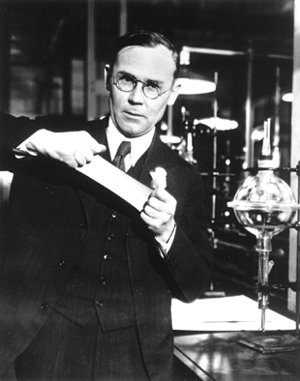
\includegraphics[width=0.24\linewidth]{images/book1/carothers.jpg}

{\small والاس كاروثرز في مختبره.}
\end{omfigure}

\section{البنية والخواص}

يمكن لعيّنتين من \omterm{def:g12:polymers:polymer}{البوليمر} نفسه أن تسلكا سلوكين مختلفين جدًا: فالمهم
طول السلاسل، وشكلها، وطريقة رصّها.

\begin{proposition}[السلاسل والخواص]\label{prop:g12:polymers:properties}
\begin{itemize}
  \item السلاسل الأطول تتشابك أكثر: فتكون المادة أمتن وتنصهر عند
        درجة حرارة أعلى.
  \item السلاسل الخطية يمكن أن تصطف جنبًا إلى جنب في مناطق منتظمة
        \emph{بلورية}؛ أما السلاسل المتفرعة فلا يمكنها ذلك، وتبقى
        غير منتظمة، \emph{لا بلورية}. والمناطق البلورية تجعل
        \omterm{def:g12:polymers:polymer}{البوليمر} أكثف وأصلب وأقل شفافية.
  \item السلاسل التي لا تمسكها جنبًا إلى جنب إلا القوى بين الجزيئية تنزلق
        بعضها على بعض حين تُسخَّن: \omterm{def:g12:polymers:polymer}{فالبوليمر} لدن حراري. أما السلاسل
        المرتبطة \emph{بجسور} تساهمية فلا تنزلق: \omterm{def:g12:polymers:polymer}{فالبوليمر}
        متصلد بالحرارة، أو، إذا قلّت الجسور، جسم صلب
        مرن كالمطاط.
\end{itemize}
\end{proposition}

\begin{proof}
يعطي التسخين السلاسل طاقة كافية للتغلب على القوى بين الجزيئية
بينها (\cref{ch:g11:polarity-and-cohesion})، وهي
أضعف من الروابط التساهمية؛ وكلما زاد التماس بين السلاسل، زادت
الطاقة اللازمة. أما الجسور فتساهمية: وكسرها يتلف
المادة بدل أن يصهرها.
\end{proof}

\begin{omfigure}
\begin{tikzpicture}[font=\footnotesize, line width=1pt, line cap=round,
    lab/.style={below, align=center, text width=2.8cm}]
  % linear, packed (crystalline)
  \begin{scope}
    \foreach \y in {0,0.25,0.5,0.75,1.0}
      \draw[omDef] plot[smooth, domain=0:2.2, samples=25] (\x, {\y + 0.05*sin(400*\x)});
    \node[lab] at (1.1,-0.2) {سلاسل خطية\\ مصطفة: بلورية};
  \end{scope}
  % linear, tangled (amorphous)
  \begin{scope}[xshift=3.4cm]
    \draw[omDef] plot[smooth] coordinates {(0,0.2) (0.5,0.9) (1.0,0.3) (1.4,1.1) (2.0,0.5) (2.2,0.9)};
    \draw[omProp] plot[smooth] coordinates {(0,0.9) (0.4,0.3) (0.9,1.0) (1.5,0.2) (1.9,1.0) (2.2,0.3)};
    \draw[black!60] plot[smooth] coordinates {(0.1,0.55) (0.7,0.1) (1.2,0.75) (1.7,0.55) (2.2,0.1)};
    \node[lab] at (1.1,-0.2) {سلاسل خطية\\ متشابكة: لا بلورية};
  \end{scope}
  % branched
  \begin{scope}[xshift=6.8cm]
    \draw[omDef] plot[smooth] coordinates {(0,0.5) (0.6,0.6) (1.2,0.45) (1.8,0.65) (2.2,0.5)};
    \draw[omDef] (0.5,0.6) -- (0.35,1.05) (1.0,0.5) -- (1.15,0.05) (1.6,0.6) -- (1.5,1.1) (1.6,0.6) -- (1.95,1.0);
    \node[lab] at (1.1,-0.2) {سلاسل متفرعة:\\ لا يمكن رصّها};
  \end{scope}
  % cross-linked
  \begin{scope}[xshift=10.2cm]
    \foreach \y in {0.1,0.55,1.0}
      \draw[omDef] plot[smooth, domain=0:2.2, samples=25] (\x, {\y + 0.06*sin(300*\x)});
    \foreach \x/\a/\b in {0.4/0.1/0.55, 1.3/0.1/0.55, 0.9/0.55/1.0, 1.9/0.55/1.0}
      \draw[omProp, line width=1.6pt] (\x,\a) -- (\x,\b);
    \node[lab] at (1.1,-0.2) {سلاسل مترابطة بجسور:\\ لا تنصهر};
  \end{scope}
\end{tikzpicture}

{\small أربعة ترتيبات لسلاسل \omterm{def:g12:polymers:polymer}{البوليمر}. والجسور (بالبرتقالي)
روابط تساهمية بين السلاسل.}
\end{omfigure}

\begin{example}[نوعان من البولي إيثين]\label{ex:g12:polymers:two-pe}
البولي إيثين المصنوع تحت ضغط مرتفع جدًا له تفرعات قصيرة كثيرة: فتُرصّ
سلاسله رصًّا سيئًا، ويعطي أغشية لينة شفافة للأكياس. أما المصنوع
بحفّاز تحت ضغط منخفض، فسلاسله شبه خطية وتُرصّ
في مناطق بلورية: فهو أكثف وأصلب، ويعطي قوارير الحليب
والصناديق. \omterm{def:g12:polymers:polymer}{المونومر} نفسه، \omterm{def:g12:polymers:repeat-unit}{والوحدة المتكررة} نفسها، لكن
البنية مختلفة.
\end{example}

\section{البوليمرات الطبيعية}

صنعت الكائنات الحية \omterm{def:g12:polymers:polymer}{البوليمرات} قبل الكيميائيين بزمن طويل.

\begin{itemize}
  \item \textbf{السليلوز} و\textbf{النشا} كلاهما سلاسل من وحدات
        الغلوكوز، \ce{C6H10O5} لكل وحدة، مرتبطة على نحو مختلف: فالسليلوز
        يكوّن أليافًا مستقيمة متينة (الخشب، القطن، الورق)؛ والنشا يكوّن
        لفائف يهضمها الجسم.
  \item \textbf{البروتينات} سلاسل من الأحماض الأمينية مرتبطة بروابط \omterm{def:g11:functional-groups:amine}{أميد}،
        هي الروابط الببتيدية في الببتيد الثنائي في
        \cref{ch:g12:synthesis-strategy}.
  \item \textbf{DNA} سلسلة من النيوكليوتيدات؛ وترتيب أنواع
        وحداته الأربعة يخزن المعلومات الوراثية.
  \item \textbf{المطاط الطبيعي} \omterm{def:g12:polymers:addition-polymer}{بوليمر إضافة} للإيزوبرين،
        \ce{CH2=C(CH3)-CH=CH2}، يُجمع على هيئة سائل لبني، اللاتكس، من
        لحاء شجرة المطاط. وإذا سُخّن مع الكبريت، ارتبطت سلاسله
        بجسور كبريتية: فيصير المطاط أمتن ويحفظ
        شكله، كما في إطار السيارة.
\end{itemize}

\begin{omfigure}
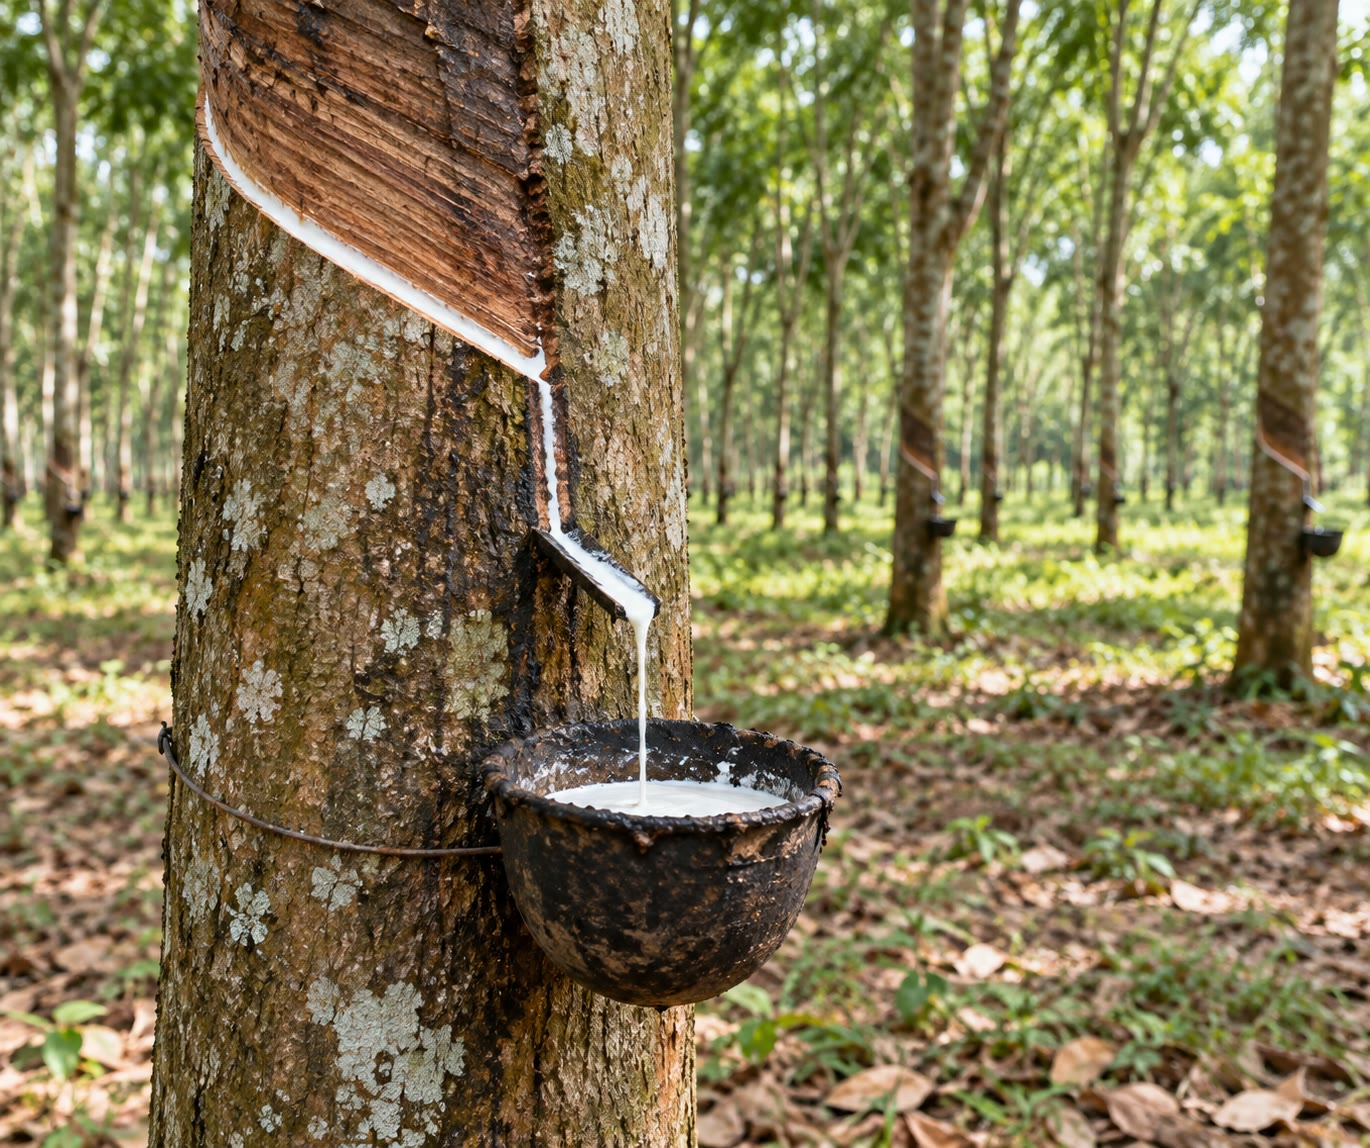
\includegraphics[width=0.45\linewidth]{images/book1/ai/g12-rubber-tapping.jpg}

{\small فصد شجرة المطاط: يسيل اللاتكس من شق في اللحاء إلى
كوب.}
\end{omfigure}

\begin{remark}[الصنع والتفكيك]\label{rem:g12:polymers:recycling}
يمكن صهر اللدن الحراري وتشكيله من جديد: وهذا هو التدوير الميكانيكي.
ويمكن أيضًا تفكيك \omterm{def:g12:polymers:addition-polymer}{بوليمر التكاثف} إلى \omterm{def:g12:polymers:polymer}{مونومراته} بالتفاعل
العكسي، أي الحلمأة، ثم صنع \omterm{def:g12:polymers:polymer}{بوليمر} جديد من المونومرات:
وهذا هو التدوير الكيميائي. أما المتصلد بالحرارة فلا يتيح أيًّا منهما بسهولة.
\end{remark}

\section{تمارين}

\begin{exercise}[$\star$]\label{exo:g12:polymers:1}
أعطِ \omterm{def:g12:polymers:polymer}{مونومر} البولي بروبين، الذي وحدته المتكررة
\ce{-CH2-CH(CH3)-}.
\end{exercise}

\begin{exercise}[$\star$]\label{exo:g12:polymers:2}
اكتب \omterm{def:g12:polymers:repeat-unit}{الوحدة المتكررة} \omterm{def:g12:polymers:polymer}{للبوليمر} المصنوع من رباعي فلورو الإيثين،
\ce{CF2=CF2}. أهو \omterm{def:g12:polymers:addition-polymer}{بوليمر إضافة} أم تكاثف؟
\end{exercise}

\begin{exercise}[$\star$]\label{exo:g12:polymers:3}
صنّف بين \omterm{def:g12:polymers:polymer}{بوليمرات} إضافة \omterm{def:g12:polymers:polymer}{وبوليمرات} تكاثف: البولي إيثين، وPET، والنايلون،
وPVC، والبوليستيرين.
\end{exercise}

\begin{exercise}[$\star$]\label{exo:g12:polymers:4}
أي هذه \omterm{def:g12:polymers:polymer}{البوليمرات} طبيعي: السليلوز، والنايلون، والنشا، وPVC،
ومطاط اللاتكس، والبروتينات؟
\end{exercise}

\begin{exercise}[$\star$]\label{exo:g12:polymers:5}
لماذا يجب أن يحمل كل \omterm{def:g12:polymers:polymer}{مونومر} من مونومرات \omterm{def:g12:polymers:addition-polymer}{بوليمر التكاثف} مجموعتين
متفاعلتين؟
\end{exercise}

\begin{exercise}[$\star\star$]\label{exo:g12:polymers:6}
لعيّنة من PVC \omterm{def:g10:the-mole:molar-mass}{كتلة مولية} متوسطة قدرها \qty{125000}{g/mol}.
احسب \omterm{def:g12:polymers:repeat-unit}{درجة بلمرتها}.
\end{exercise}

\begin{exercise}[$\star\star$]\label{exo:g12:polymers:7}
لسلسلة من البوليستيرين درجة \omterm{def:g12:polymers:polymer}{بلمرة} قدرها 2500. احسب
كتلتها المولية.
\end{exercise}

\begin{exercise}[$\star\star$]\label{exo:g12:polymers:8}
يحمل حمض اللبنيك، \ce{CH3-CH(OH)-COOH}، مجموعة كحولية ومجموعة
حمضية. بيّن أنه يستطيع تكوين بوليستر وحده، واكتب وحدته
المتكررة، وسمِّ \omterm{def:g7:atoms-and-molecules:molecule}{الجزيء} الصغير المنطلق.
\end{exercise}

\begin{exercise}[$\star\star$]\label{exo:g12:polymers:9}
اشرح، مستعينًا بشكل ترتيبات السلاسل، لماذا تكون أغشية الأكياس لينة
وشفافة بينما تكون قوارير الحليب صلبة ومعتمة.
\end{exercise}

\begin{exercise}[$\star\star$]\label{exo:g12:polymers:10}
مقبض المقلاة متصلد بالحرارة، وكذلك مقبض غطائها البلاستيكي. صف
سلاسلهما. ولماذا لا يمكن صهرهما وتدويرهما؟
\end{exercise}

\begin{exercise}[$\star\star$]\label{exo:g12:polymers:11}
لسلسلة من النايلون 6,6 \omterm{def:g10:the-mole:molar-mass}{كتلة مولية} قدرها \qty{22600}{g/mol}. احسب
\omterm{def:g10:the-mole:molar-mass}{الكتلة المولية} لوحدتها المتكررة \ce{C12H22N2O2}، ثم \omterm{def:g12:polymers:repeat-unit}{درجة
بلمرتها}.
\end{exercise}

\begin{exercise}[$\star\star\star$]\label{exo:g12:polymers:12}
اكتب التفاعل بين \omterm{def:g7:atoms-and-molecules:molecule}{جزيء} من الهكسان-1,6-ثنائي \omterm{def:g11:functional-groups:amine}{أمين} \omterm{def:g7:atoms-and-molecules:molecule}{وجزيء} من
حمض الهكسان ديويك، الذي يعطي أول رابطة \omterm{def:g11:functional-groups:amine}{أميد}. ولماذا يستطيع \omterm{def:g7:chemical-reactions:reactant}{الناتج} أن يستمر في
التفاعل من طرفيه؟
\end{exercise}

\begin{exercise}[$\star\star\star$]\label{exo:g12:polymers:13}
ما كتلة الماء المنطلقة حين يُصنع \qty{1.0}{kg} من النايلون 6,6؟
\end{exercise}

\begin{exercise}[$\star\star\star$]\label{exo:g12:polymers:14}
المطاط الطبيعي لين ولزج حين يكون دافئًا؛ وإذا سُخّن مع الكبريت،
صار المطاط المرن المتين في الإطارات. اشرح ذلك بالسلاسل.
ولماذا يصعب تدوير الإطار إلى هذا الحد؟
\end{exercise}

\begin{exercise}[$\star\star\star$]\label{exo:g12:polymers:15}
للنشا والسليلوز الصيغة نفسها لكل وحدة، \ce{C6H10O5}. ولسلسلة
سليلوز \omterm{def:g10:the-mole:molar-mass}{كتلة مولية} قدرها \qty{1.6e6}{g/mol}. كم وحدة غلوكوز
تحوي؟ وكم طولها، إذا كانت كل وحدة تضيف \qty{0.5}{nm} إلى
طولها؟
\end{exercise}

\section{مسألة: من القارورة إلى السترة الصوفية}

\begin{problem}[{مسألة نهاية الأسبوع --- كم قارورة كتلتها 25 g تدخل في
سترة صوفية صناعية واحدة؟}]
\label{pb:g12:polymers:1}
% ledger: aw:C, aw:H, aw:O
تُصنع سترة صوفية صناعية من \qty{300}{g} من ألياف PET. وتُجمع قوارير مستعملة
كتلة كل منها \qty{25}{g}، وتُفرز وتُغسل وتُفرم وتُصهر وتُغزل؛
وفي هذه العملية تنتهي \qty{80}{\percent} من كتلة القوارير أليافًا
في السترة.

\medskip
\noindent\textbf{الجزء الأول --- \omterm{def:g12:polymers:polymer}{البوليمر}.}
\begin{enumerate}
  \item سمِّ مونومري PET والمجموعات الوظيفية التي
        يحملانها.
  \item أي رابطة تتكوّن بينهما؟ وأي \omterm{def:g7:atoms-and-molecules:molecule}{جزيء} صغير ينطلق؟
  \item أPET \omterm{def:g12:polymers:addition-polymer}{بوليمر إضافة} أم \omterm{def:g12:polymers:addition-polymer}{بوليمر تكاثف}؟
  \item احسب الكتلتين الموليتين للمونومرين.
  \item استنتج \omterm{def:g10:the-mole:molar-mass}{الكتلة المولية} \omterm{def:g12:polymers:repeat-unit}{للوحدة المتكررة} \ce{C10H8O4}، وتحقق
        منها بصيغتها.
\end{enumerate}

\medskip
\noindent\textbf{الجزء الثاني --- السلاسل.}
\begin{enumerate}[resume]
  \item لمادة PET في القوارير سلاسل كتلتها المولية المتوسطة
        \qty{38400}{g/mol}. احسب \omterm{def:g12:polymers:repeat-unit}{درجة البلمرة}.
  \item كم رابطة \omterm{def:g11:functional-groups:carboxylic-acid}{إستر} تحوي السلسلة الواحدة، تقريبًا؟
  \item PET القوارير بلوري جزئيًا. فماذا يقول ذلك عن
        سلاسله؟
  \item لماذا يمكن صهر PET وغزله أليافًا؟
\end{enumerate}

\medskip
\noindent\textbf{الجزء الثالث --- التدوير.}
\begin{enumerate}[resume]
  \item ما كتلة القوارير اللازمة لسترة واحدة؟
  \item كم قارورة يمثل ذلك؟
  \item ماذا يحدث لبقية الكتلة؟
  \item أي مبدأ من مبادئ \omterm{def:g12:synthesis-strategy:green-chemistry}{الكيمياء الخضراء} يطبّق هذا التدوير؟
\end{enumerate}

\medskip
\noindent\textbf{الجزء الرابع --- العودة إلى المونومرات.}
\begin{enumerate}[resume]
  \item اكتب، \omterm{def:g12:polymers:repeat-unit}{لوحدة متكررة} واحدة، حلمأة PET إلى
        مونومريه.
  \item ما كمية الوحدات المتكررة في \qty{1.00}{kg} من PET؟
  \item ما كتلتا المونومرين اللتان تعطيهما الحلمأة الكاملة
        لكتلة \qty{1.00}{kg} من PET؟
  \item ما كتلة الماء التي تستهلكها؟ وتحقق من انحفاظ
        الكتلة.
  \item أعطِ ميزة واحدة لهذا التدوير الكيميائي على الصهر.
  \item اذكر الجواب النهائي: كم قارورة كتلتها \qty{25}{g} تدخل في
        سترة صوفية صناعية واحدة؟
\end{enumerate}
\end{problem}
